\documentclass{article}
\usepackage{tikz} 
\usepackage[utf8]{inputenc}
\usepackage{amsmath}
\usepackage{listings}
\usepackage{amsfonts}
\usepackage{amssymb}
\usepackage{tabularx}
\usepackage{enumitem}
\usepackage{algorithm}% http://ctan.org/pkg/algorithm
\usepackage[noend]{algpseudocode}% http://ctan.org/pkg/algorithmicx
\usepackage{tikz}
\usepackage{graphicx}


\usepackage{subcaption}
\usepackage{multicol,caption}
\usepackage{geometry}
 \geometry{
 a4paper,
 total={210mm,297mm},
 left=20mm,
 right=20mm,
 top=20mm,
 bottom=20mm,
 }

\usetikzlibrary{arrows,positioning,shapes,fit} 
\pgfarrowsdeclarecombine{ring}{ring}{}{}{o}{o}
\thispagestyle{empty}
\DeclareMathOperator{\ringarrow}{\raisebox{0.5ex}{\tikz[baseline]{\draw[ring->](0,0)--(2em,0);}}}

\definecolor{talk}{HTML}{729FCF}
\definecolor{talk2}{HTML}{E8A753}
\definecolor{grey}{HTML}{DBDCDD}
\renewcommand{\vec}[1]{\boldsymbol{#1}}
\tikzset{
    %Define standard arrow tip
    >=stealth',
    %Define style for boxes
    observed/.style={
   	circle,
   	rounded corners,
   	draw=black, thick,
   	minimum width=2.3em,
   	minimum height=2.3em,
   	font=\footnotesize,
   	text centered,
   	fill=talk!50
   },
   latent/.style={
   	circle,
   	rounded corners,
   	draw=black, thick, dashed,
   	minimum width=2.2em,
   	minimum height=2.2em,
   	font=\footnotesize,
   	text centered
   },
    % Define arrow style
    pil/.style={
           o->,
           thick,
           shorten <=2pt,
           shorten >=2pt,},
    sh/.style={ shade, shading=axis, left color=red, right color=green,
    shading angle=45 },
observedrect/.style={
	rectangle,
	rounded corners,
	draw=black, thick,
	minimum width=3em,
	minimum height=1.5em,
	font=\footnotesize,
	text centered,
	fill=talk2!80
},  
 target/.style={
	circle,
	rounded corners,
	draw=black, thick,
	minimum width=2.3em,
	minimum height=2.3em,
	font=\footnotesize,
	text centered,
	fill=talk2!80
},
empty/.style={
	circle,
	rounded corners,
	minimum width=.5em,
	minimum height=.5em,
	font=\footnotesize,
	text centered,
},
}
   
\begin{document}
%\pagestyle{empty}

 \begin{figure}[ht]
 	\begin{subfigure}[t]{0.49\textwidth}
 		\centering    
 		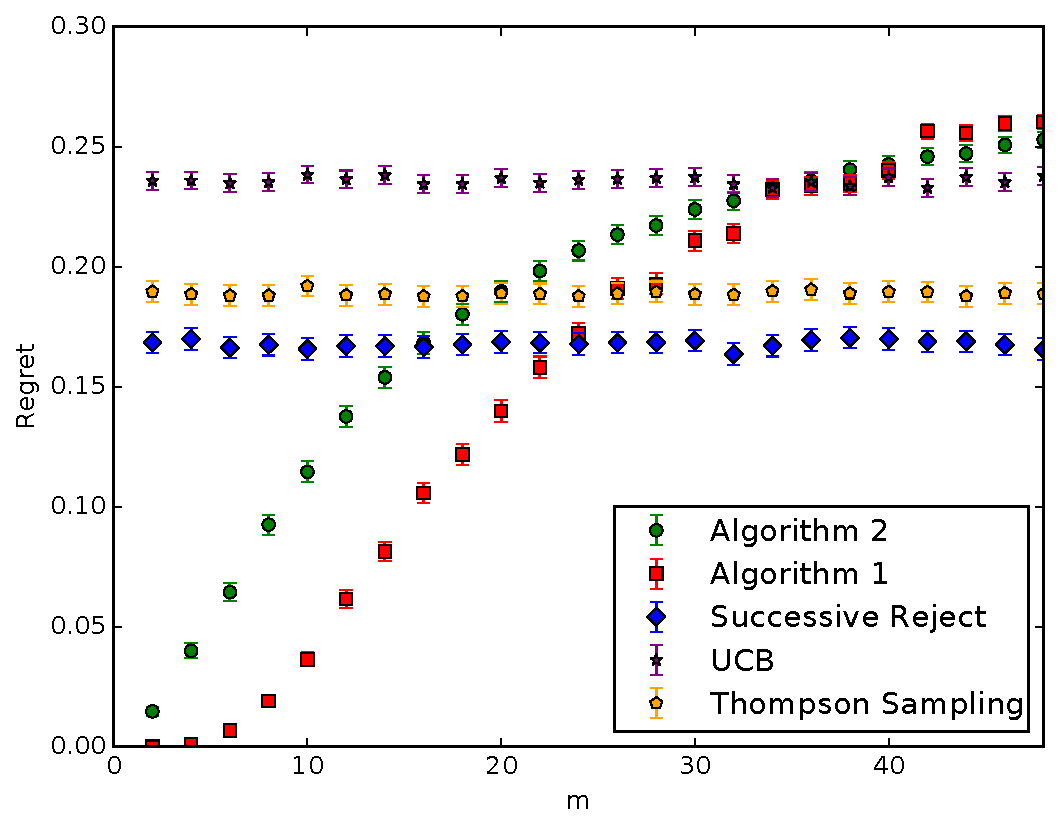
\includegraphics[width=\textwidth]{experiment1_20161020_1247.pdf}
 		\caption{Simple regret vs $m(\boldsymbol{q})$ for fixed horizon $T=400$ and number of variables $N = 50$}
 		\label{fig:simple_vs_m}
 	\end{subfigure}\hfill
 	\begin{subfigure}[t]{0.49\textwidth}
 		\centering
 		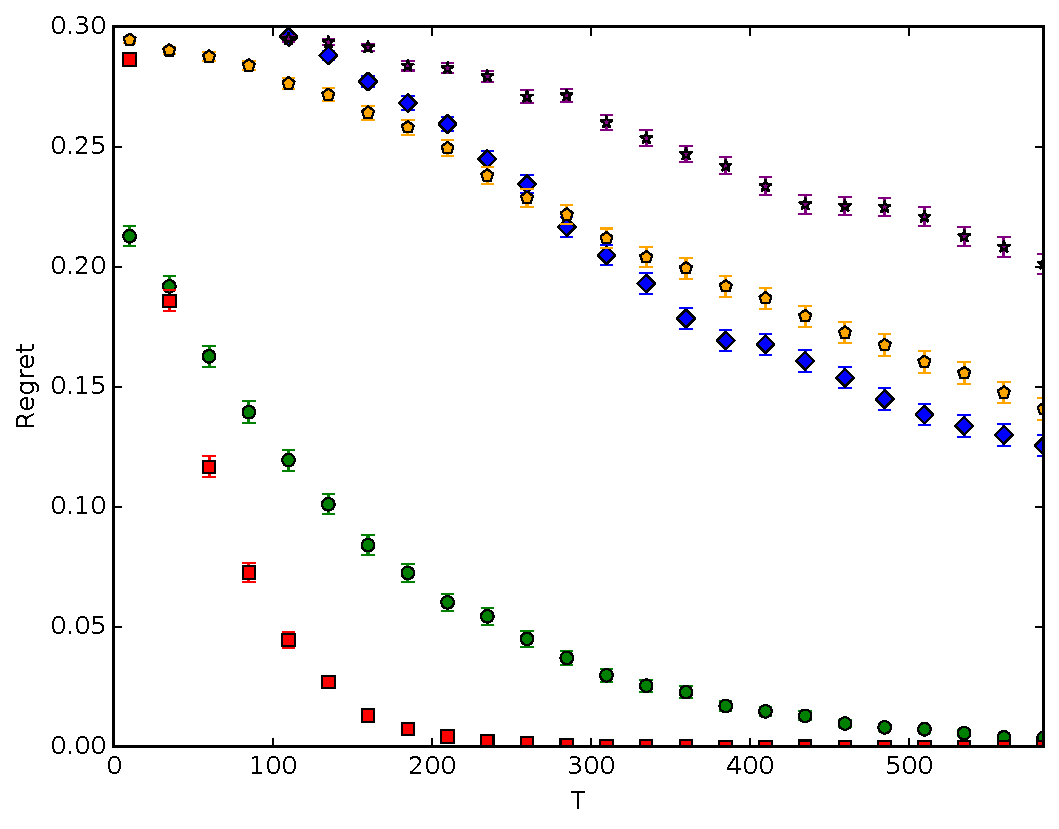
\includegraphics[width=\textwidth]{experiment3_20161020_1252.pdf}
 		\caption{Simple regret vs horizon, $T$, with $N = 50$, $m=2$ and fixed $\epsilon = .3$}
 		\label{fig:simple_vs_T}
 	\end{subfigure}
 \end{figure}

\end{document}